% =====================================================================
%  Treść — Warsaw Civic Budget 2027: raport empiryczny seed datasetu
% =====================================================================

\begin{abstract}
\noindent
Budujemy seed datasetu języka współczesnej polszczyzny z opisów projektów
Budżetu Obywatelskiego Warszawy~2027 (licencja CC~BY-SA~4.0).
Aktualny stan: 89~rekordów, 152\,526~znaków, 9~kategorii, 16~dzielnic;
80~pełnych kart ze stabilnym \texttt{source\_url} i~kompletną atrybucją.
Analiza redundancji wykazała medianę podobieństwa TF-IDF $= 0{,}034$
w~rdzeniu pełnych kart --- poziom niski, porównywalny z~niezależnymi
dokumentami. Seed spełnia kryteria recenzji v0.1, lecz nie jest jeszcze
dojrzałym datassetem produkcyjnym.
\end{abstract}

% ---------------------------------------------------------------
\section{Wprowadzenie}

\textbf{Pytanie:} czy opisy projektów Budżetu Obywatelskiego Warszawy~2027
dostarczają reprezentatywny i~nieredundantny zbiór języka codziennej
polszczyzny, przydatny jako materiał treningowy dla Slayera?

\smallskip
\noindent
Nitka dialektyczna:

\medskip
\noindent
\textbf{Teza~(T):} Zbiór 80~pełnych kart (149\,657~znaków tekstu z~kart)
o~tematyce zdrowia, edukacji, sportu i~transportu tworzy audytowalny,
licencjonowany seed języka codziennej polszczyzny.

\medskip
\noindent
\textbf{Antyteza~(A):} Dziewięć krótkich rekordów listowych
(mediana TF-IDF $= 0{,}452$) i~jedna para wysokiego ryzyka
(studnie oligoceńskie, TF-IDF $= 0{,}679$) osłabiają jednorodność
zbioru; seed NIE jest gotowy do treningu produkcyjnego.

\medskip
\noindent
\textbf{Synteza~(S):} Rdzeń 80~pełnych kart przechodzi wszystkie
kontrole jakości (zero duplikatów, zero danych kontaktowych,
atrybucja 80/80). Usunięcie 9~rekordów listowych i~karty-duplikatu
studni $(\approx 2{,}55\%$ znaków) eliminuje główne ryzyko redundancji
i~otwiera drogę do wydania gotowego do recenzji zespołu.

% ---------------------------------------------------------------
\section{Metoda}

\subsection*{Źródło i licencja}
Dane pochodzą z~platformy Budżetu Obywatelskiego Warszawy~2027.
Strona platformy wskazuje licencję Creative Commons~BY-SA~4.0%
\footnote{\url{https://creativecommons.org/licenses/by-sa/4.0/}}.
Każdy rekord zachowuje konkretny \texttt{source\_url},
\texttt{license\_url} i~datę pobrania; atrybucja twórców przechowywana
jest oddzielnie od tekstu treningowego.

\subsection*{Ekstrakcja i czyszczenie}
Rekordy pozyskiwano ręcznie lub półautomatycznie z~kart szczegółowych
projektów (\texttt{detail\_seed}). Dziewięć wcześniejszych rekordów
pochodzi z~widoku listy (\texttt{list\_seed}) i~zawiera słabsze opisy.
Czyszczenie: usunięcie tagów~HTML, zastąpienie numerów telefonów
i~adresów e-mail znacznikiem \texttt{[usunięto dane kontaktowe]},
wykluczenie rekordów zbyt krótkich ($< 50$~znaków). Styl językowy
wnioskodawców został zachowany bez wygładzania.

\subsection*{Deduplikacja i analiza redundancji}
Duplikaty identyfikowane kluczem tekstowym. Podobieństwo par rekordów
mierzone dwiema metrykami:
\[
  \mathrm{sim}_{\cos}(d_i, d_j)
    = \frac{\mathbf{v}_i \cdot \mathbf{v}_j}
           {\|\mathbf{v}_i\| \cdot \|\mathbf{v}_j\|}
\]
gdzie $\mathbf{v}_k$ to wektor TF-IDF dokumentu $d_k$ na słowach
treściowych, oraz podobieństwo Jaccarda na~5-gramach wyrazowych:
\[
  J_5(d_i, d_j)
    = \frac{|G_5(d_i) \cap G_5(d_j)|}
           {|G_5(d_i) \cup G_5(d_j)|}
\]

% ---------------------------------------------------------------
\section{Wyniki}

\subsection*{Stan ogólny}

\begin{table}[h]
  \centering
  \caption{Podsumowanie zbioru Warsaw Civic Budget 2027.}
  \label{tab:summary}
  \begin{tabular}{lr}
    \toprule
    Metryka                          & Wartość \\
    \midrule
    Rekordy treningowe               & 89 \\
    Znaki tekstu treningowego        & 152\,526 \\
    Pełne karty (\texttt{detail})    & 80 \\
    \quad z czego znaki              & 149\,657 \\
    Rekordy listowe (\texttt{list})  & 9 \\
    \quad z czego znaki              & 2\,869 \\
    Kategorie                        & 9 \\
    Dzielnice / poziomy              & 16 \\
    Najkrótszy tekst [znaki]         & 235 \\
    Najdłuższy tekst [znaki]         & 2\,981 \\
    Brakujące pola (detail)          & 0 / 8 pól \\
    Dane kontaktowe w tekście        & 0 \\
    Duplikaty po deduplikacji        & 0 \\
    Atrybucja pełnych kart           & 80 / 80 \\
    \bottomrule
  \end{tabular}
\end{table}

\subsection*{Redundancja}

\begin{table}[h]
  \centering
  \caption{Porównanie redundancji warstw danych (TF-IDF/kosinus,
  5-gramy Jaccarda).}
  \label{tab:redundancy}
  \begin{tabular}{lrrrrr}
    \toprule
    Warstwa & Rek. & Znaki & Med.\ sim. & Śr.\ sim.
            & Pary $\ge 0{,}50$ \\
    \midrule
    Pełne karty  & 80 & 149\,657 & 0{,}034 & 0{,}036 & 0 \\
    Rek.\ listowe &  9 &   2\,869 & 0{,}452 & 0{,}511 & 12 \\
    \bottomrule
  \end{tabular}
\end{table}

Jedyna para wysokiego ryzyka w~pełnych kartach to dwa projekty studni
oligoceńskich: TF-IDF $= 0{,}679$, Jaccard$_5 = 0{,}269$.
Rekomendacja: usunąć krótszą kartę (ul.~Kołacińska, $\approx 1\,016$~znaków).

\subsection*{Status projektów}

\begin{figure}[h]
  \centering
  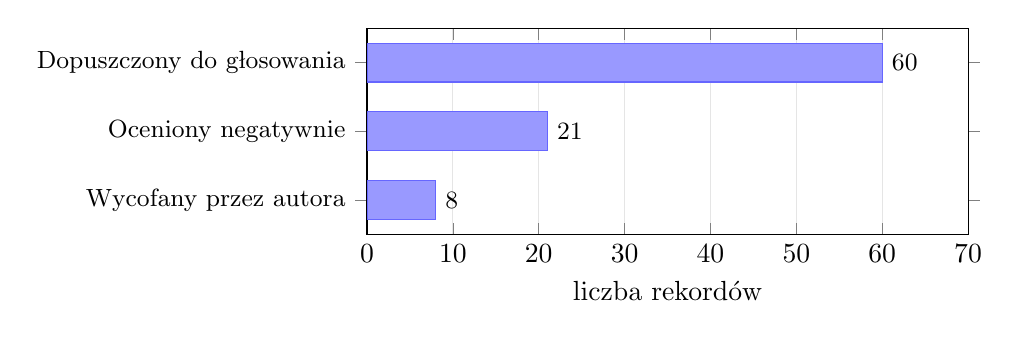
\begin{tikzpicture}
    \begin{axis}[
        xbar, bar width=14pt,
        width=0.76\linewidth, height=4.2cm,
        symbolic y coords={wycofany, negatywny, dopuszczony},
        ytick=data,
        yticklabels={Wycofany przez autora, Oceniony negatywnie,
                     Dopuszczony do głosowania},
        xlabel={liczba rekordów},
        xmin=0, xmax=70,
        nodes near coords, nodes near coords align={horizontal},
        every node near coord/.style={font=\small},
        xmajorgrids=true, grid style={gray!20},
        y tick label style={font=\small},
        enlarge y limits=0.25,
    ]
      \addplot[fill=blue!40, draw=blue!60] coordinates {
        (8,wycofany)
        (21,negatywny)
        (60,dopuszczony)
      };
    \end{axis}
  \end{tikzpicture}
  \caption{Rozkład statusów 89~rekordów. 60~projektów dopuszczonych
  do głosowania (67{,}4\%), 21~ocenionych negatywnie (23{,}6\%),
  8~wycofanych przez autora (9{,}0\%).
  Uzasadnienia negatywnych ocen wzbogacają zbiór o~rzadki rejestr
  urzędniczej polszczyzny.}
  \label{fig:status}
\end{figure}

Odwołania: rys.~\ref{fig:hero} (rozkład kategorii),
rys.~\ref{fig:status} (statusy), tab.~\ref{tab:summary},
tab.~\ref{tab:redundancy}.

% ---------------------------------------------------------------
\section{Warunek obalenia}

Teza o~niskiej redundancji rdzenia pełnych kart upada, jeśli
spełniony zostanie którykolwiek z~poniższych warunków:

\begin{enumerate}
  \item Liczba par pełnych kart z~TF-IDF $\ge 0{,}50$ przekroczy
        $1\%$ wszystkich par, czyli $> 31$ par spośród
        $\binom{80}{2} = 3\,160$. Aktualnie: \textbf{0~par}.
  \item Odsetek rekordów z~brakującym \texttt{license\_url}
        wśród pełnych kart (detail) przekroczy $0\%$.
        Aktualnie: \textbf{0~brakujących / 80}.
  \item Walidator wykryje dane kontaktowe w~tekście treningowym.
        Aktualnie: \textbf{0~trafień}.
\end{enumerate}

Żaden z~warunków nie jest spełniony --- synteza nie zostaje obalona.

% ---------------------------------------------------------------
\section{Dyskusja}

\textbf{Ograniczenia.} Seed pochodzi wyłącznie z~jednego miasta
(Warszawa) i~jednej edycji (2027), co ogranicza geograficzną
i~czasową różnorodność. Kategorie są nierównomiernie reprezentowane:
zdrowie dominuje (19~rek.), ochrona środowiska jest niedoreprezentowana
(4~rek.). Dziewięć rekordów listowych wnosi metadane, lecz słabe opisy
tekstowe --- ich wartość treningowa jest istotnie niższa od pełnych kart
(mediana TF-IDF $= 0{,}452$ vs $0{,}034$).

\textbf{Co dalej.} Trzy priorytety kolejnego etapu:
(1)~usunąć lub zastąpić 9~rekordów listowych pełnymi kartami,
(2)~usunąć kartę studni przy ul.~Kołacińskiej (TF-IDF $= 0{,}679$),
(3)~wyrównać kategorie przez dobór kart z~ochrony środowiska,
komunikacji i~kultury. Po korekcie szacowana strata to
$\approx 3\,885$~znaków $(2{,}55\%$ zbioru), a~zysk to
wyraźnie czystszy i~jednorodniejszy rdzeń treningowy.

% ---------------------------------------------------------------
\section*{Podpis}
Dokument autorstwa: \emph{PiotrStyla}. Dane: CC~BY-SA~4.0,
Budżet Obywatelski Warszawy~2027.
Skompilowany w~CI (\texttt{.tex}~$\to$~PDF, artefakt \texttt{raport-pdf}).
Data: \today.
